\documentclass[12pt,a4paper]{report}

% ─── Packages ───────────────────────────────────────────────────────────────
\usepackage[top=2.5cm, bottom=2.5cm, left=2.8cm, right=2.8cm]{geometry}
\usepackage[T1]{fontenc}
\usepackage[utf8]{inputenc}
\usepackage{lmodern}
\usepackage{microtype}
\usepackage{xcolor}
\usepackage{booktabs}
\usepackage{longtable}
\usepackage{array}
\usepackage{multirow}
\usepackage{graphicx}
\usepackage{tikz}
\usetikzlibrary{shapes.geometric, arrows.meta, positioning, fit, calc, backgrounds}
\usepackage{hyperref}
\usepackage{enumitem}
\usepackage{fancyhdr}
\usepackage{titlesec}
\usepackage{caption}
\usepackage{subcaption}
\usepackage{amsmath}
\usepackage{listings}
\usepackage{setspace}
\usepackage{parskip}
\usepackage{tocloft}
\usepackage{emptypage}

% ─── Colours ────────────────────────────────────────────────────────────────
\definecolor{accent}{RGB}{109,40,217}
\definecolor{accentlight}{RGB}{167,139,250}
\definecolor{darkbg}{RGB}{3,7,18}
\definecolor{codered}{RGB}{220,38,38}
\definecolor{codegreen}{RGB}{22,163,74}
\definecolor{codegray}{RGB}{107,114,128}
\definecolor{rowalt}{RGB}{245,243,255}
\definecolor{tableheader}{RGB}{109,40,217}

% ─── Hyperref ───────────────────────────────────────────────────────────────
\hypersetup{
  colorlinks   = true,
  linkcolor    = accent,
  urlcolor     = accentlight,
  citecolor    = accent,
  pdftitle     = {MindMonitor --- System Architecture \& Technical Reference},
  pdfauthor    = {MindMonitor Engineering},
  pdfsubject   = {Software Architecture Documentation},
}

% ─── Section formatting ─────────────────────────────────────────────────────
\titleformat{\chapter}[hang]
  {\Large\bfseries\color{accent}}
  {\thechapter.}{0.8em}{}[\vspace{-0.3em}\rule{\textwidth}{0.4pt}]

\titleformat{\section}
  {\large\bfseries\color{accent!85!black}}
  {\thesection}{0.7em}{}

\titleformat{\subsection}
  {\normalsize\bfseries\color{accent!70!black}}
  {\thesubsection}{0.6em}{}

\titleformat{\subsubsection}
  {\normalsize\itshape\color{codegray}}
  {\thesubsubsection}{0.5em}{}

% ─── Header / Footer ────────────────────────────────────────────────────────
\pagestyle{fancy}
\fancyhf{}
\fancyhead[L]{\small\color{codegray}\textit{MindMonitor --- Technical Architecture Reference}}
\fancyhead[R]{\small\color{codegray}\thepage}
\renewcommand{\headrulewidth}{0.3pt}
\renewcommand{\headrule}{\hbox to\headwidth{\color{accentlight}\leaders\hrule height \headrulewidth\hfill}}

% ─── Listings style ─────────────────────────────────────────────────────────
\lstset{
  basicstyle   = \ttfamily\footnotesize,
  keywordstyle = \color{accent}\bfseries,
  commentstyle = \color{codegray}\itshape,
  stringstyle  = \color{codegreen},
  breaklines   = true,
  frame        = single,
  framerule    = 0.4pt,
  rulecolor    = \color{accentlight},
  xleftmargin  = 1em,
  xrightmargin = 1em,
}

% ─── Table helpers ──────────────────────────────────────────────────────────
\newcolumntype{L}[1]{>{\raggedright\arraybackslash}p{#1}}
\newcolumntype{C}[1]{>{\centering\arraybackslash}p{#1}}

% ─── TikZ styles ────────────────────────────────────────────────────────────
\tikzset{
  block/.style    = {rectangle, rounded corners=4pt, draw=accent, fill=rowalt,
                     text width=#1, align=center, minimum height=1cm,
                     font=\small\bfseries},
  block/.default  = 2.8cm,
  cloud/.style    = {ellipse, draw=accent!60, fill=accent!10,
                     text width=2.4cm, align=center, minimum height=0.9cm,
                     font=\small\bfseries},
  hw/.style       = {rectangle, draw=codered!70, fill=codered!10,
                     text width=2.4cm, align=center, minimum height=0.9cm,
                     font=\small\bfseries, rounded corners=2pt},
  db/.style       = {cylinder, shape border rotate=90, draw=codegreen!70,
                     fill=codegreen!10, text width=2cm, align=center,
                     minimum height=1cm, font=\small\bfseries},
  arrow/.style    = {-Stealth, thick, color=accent},
  darrow/.style   = {Stealth-Stealth, thick, color=accent!70},
  label/.style    = {font=\tiny\color{codegray}, midway, sloped},
}

% ═══════════════════════════════════════════════════════════════════════════
\begin{document}

\begin{titlepage}
  \centering
  \vspace*{3cm}
  {\color{accent}\rule{\textwidth}{2pt}}
  \vspace{1cm}

  {\fontsize{28}{34}\selectfont\bfseries\color{accent} MindMonitor}\\[0.4em]
  {\Large\color{codegray} Mental Health Monitoring Platform}\\[0.8em]
  {\color{accentlight}\rule{8cm}{0.6pt}}\\[1em]
  {\large\bfseries System Architecture \& Technical Reference}\\[0.4em]
  {\normalsize Version 0.1.0 \quad|\quad April 2026}

  \vspace{3cm}
  \begin{tabular}{L{4cm} L{8cm}}
    \toprule
    \textbf{Category}     & \textbf{Value} \\
    \midrule
    Project Name          & MindMonitor \\
    Version               & 0.1.0 \\
    Framework             & Next.js 16.1.6 / React 19.2.3 \\
    Primary Database      & PostgreSQL via Supabase \\
    Real-time Database    & Firebase Realtime Database \\
    Hardware Platform     & Arduino Mega + ESP8266 \\
    Document Date         & April 2026 \\
    \bottomrule
  \end{tabular}

  \vfill
  {\color{accent}\rule{\textwidth}{2pt}}
\end{titlepage}

\tableofcontents
\clearpage

% ═══════════════════════════════════════════════════════════════════════════
\chapter{Project Overview \& Architectural Summary}
\label{ch:overview}

\section{System Description}

MindMonitor is a full-stack mental health monitoring platform that bridges
IoT sensor hardware with a multi-role web application. The system collects
physiological data (GSR, heart rate, SpO2, skin temperature) from a
patient-worn sensor node and delivers real-time stress analysis, anomaly
alerts, and clinician-facing dashboards via a Next.js application backed
by a dual-database architecture.

The platform is structured around two distinct user personas: \textbf{patients},
who wear the sensor hardware and view their own biometric trends, and
\textbf{doctors}, who monitor assigned patient data, trigger video consultations,
and submit clinical evaluations. All data pathways---from hardware to browser---are
fully asynchronous and event-driven.

\section{Architectural Patterns}

\begin{itemize}[leftmargin=1.5em]
  \item \textbf{Hybrid SSR + SPA}: Next.js App Router delivers server-rendered
        shells with client-side hydration for interactive dashboard panels.
        Protected routes are enforced by server-side middleware before any
        page component executes.

  \item \textbf{IoT-Edge-to-Cloud Sync}: A two-chip hardware node
        (Arduino Mega for sensing, ESP8266 for connectivity) pushes readings
        over serial CSV to Firebase Realtime Database. The browser subscribes
        directly to Firebase listeners; a secondary pipeline persists readings
        into PostgreSQL for longitudinal storage.

  \item \textbf{Dual-Database Persistence}: Firebase RTDB acts as the
        low-latency, high-availability real-time bus; Supabase-hosted PostgreSQL
        serves as the system-of-record for analytics, evaluations, alerts, and
        appointments. Prisma ORM mediates all PostgreSQL access.

  \item \textbf{Role-Based Access Control (RBAC)}: Supabase Auth manages
        identity. A Next.js edge middleware layer inspects JWT claims to enforce
        route-level access separation between \texttt{PATIENT} and
        \texttt{DOCTOR} roles before page rendering begins.

  \item \textbf{Event-Driven Alerting}: Anomaly rules execute synchronously
        at the ingestion boundary. Qualifying readings atomically produce
        \texttt{Alert} records visible to both roles in real time.
\end{itemize}

\section{Key Design Decisions}

\begin{enumerate}[leftmargin=1.5em]
  \item \textbf{Firebase as real-time bus, PostgreSQL as record store}:
        Firebase's WebSocket-backed listeners eliminate polling for live
        dashboards; PostgreSQL provides SQL-queryable history, joins, and
        transactional integrity for clinical records.

  \item \textbf{Client-side Firebase subscription with server-side ingestion}:
        The \texttt{useSessionStream} hook subscribes to Firebase in the browser
        and mirrors each new reading to \texttt{/api/readings/ingest}, which
        deduplicates and writes to Postgres. This decouples the real-time
        display path from the persistence path.

  \item \textbf{ZegoCloud UIKit for video}: Rather than building custom WebRTC
        signaling, the platform uses ZegoCloud's prebuilt UIKit component,
        reducing implementation surface while retaining room-level control
        (\texttt{roomId} stored per appointment in PostgreSQL).

  \item \textbf{Serial CSV bridge between Arduino and ESP8266}: The
        microcontroller-level split keeps sensor firmware independent of
        network credentials and Firebase SDK complexity. Only the ESP8266
        runs the network stack.
\end{enumerate}

% ═══════════════════════════════════════════════════════════════════════════
\chapter{Technology Stack}
\label{ch:stack}

\begin{longtable}{L{2.4cm} L{3.2cm} L{3.0cm} L{6.2cm}}
  \caption{Complete Technology Stack\label{tab:stack}} \\
  \toprule
  \rowcolor{tableheader}
  \color{white}\textbf{Layer} &
  \color{white}\textbf{Technology} &
  \color{white}\textbf{Purpose} &
  \color{white}\textbf{Project-Specific Mechanics} \\
  \midrule
  \endfirsthead

  \multicolumn{4}{c}{\textit{(continued from previous page)}} \\
  \toprule
  \rowcolor{tableheader}
  \color{white}\textbf{Layer} &
  \color{white}\textbf{Technology} &
  \color{white}\textbf{Purpose} &
  \color{white}\textbf{Project-Specific Mechanics} \\
  \midrule
  \endhead

  \bottomrule
  \endfoot

  \rowcolor{rowalt}
  Frontend & Next.js 16.1.6 & SSR framework, routing, API layer &
    App Router with route groups \texttt{(auth)}, \texttt{(patient)},
    \texttt{(doctor)}. Server Components render page shells; Client
    Components hydrate charts and live data panels. \\

  Frontend & React 19.2.3 & UI rendering &
    Concurrent mode enabled. Client Components subscribe to Firebase
    listeners and manage local optimistic state for chart updates. \\

  \rowcolor{rowalt}
  Frontend & TypeScript 5 & Type safety &
    Strict mode. Prisma-generated types propagate from ORM layer to
    API response shapes and component props via shared interfaces. \\

  Frontend & Tailwind CSS v4 & Utility-first styling &
    PostCSS plugin integration. Dark design system: \texttt{bg-gray-950}
    base, glassmorphism card primitives, violet accent (\texttt{\#6D28D9})
    throughout. \\

  \rowcolor{rowalt}
  Frontend & Framer Motion 12 & Animation &
    Entry animations on login, dashboard panels, and landing page
    sections. Used for staggered card reveals and hover transitions. \\

  Frontend & Recharts 3.7 & Data visualisation &
    \texttt{StressLineChart}, \texttt{VitalsLineChart}, \texttt{GsrLineChart},
    \texttt{StressDistributionPie}, \texttt{TemperatureGauge} components.
    Fed from both live Firebase state and historical PostgreSQL queries. \\

  \rowcolor{rowalt}
  Backend & Next.js API Routes & REST API server &
    All endpoints under \texttt{src/app/api/}. No separate server process;
    API routes run as Node.js serverless functions on Vercel or as part of
    the Next.js server process in self-hosted mode. \\

  Backend & Node.js 20 & Runtime &
    Hosts Prisma client, Firebase Admin SDK calls (via REST), serial
    port bridge utilities. \texttt{serialport} package v13 used for
    hardware ingestion bridge in \texttt{bridge/} directory. \\

  \rowcolor{rowalt}
  Database & PostgreSQL (Supabase) & Primary data store &
    Two connection strings: pooler URL (\texttt{port 6543},
    \texttt{pgbouncer=true}) for application queries; direct URL
    (\texttt{port 5432}) for Prisma migrations. Connection pool
    managed by PgBouncer in transaction mode. \\

  ORM & Prisma 6.19 & Schema management, query builder &
    Singleton client instantiated in \texttt{src/lib/prisma.ts} with
    global reference to survive HMR restarts. \texttt{log: ["error"]}
    in production. Generates TypeScript types from schema. \\

  \rowcolor{rowalt}
  Real-time & Firebase RTDB 12 & Low-latency sensor bus &
    Hosted in \texttt{asia-southeast1} region. Browser SDK attaches
    \texttt{onValue} listeners to \texttt{/live/current/\{sessionId\}}.
    ESP8266 writes via authenticated REST calls (PATCH/POST). \\

  Real-time & Firebase REST API & Server-side RTDB writes &
    \texttt{src/lib/firebaseRtdbServer.ts} issues
    \texttt{fetch} calls to the RTDB REST endpoint, using
    \texttt{access\_token=...} query parameter for auth. \\

  \rowcolor{rowalt}
  Auth & Supabase Auth & Identity management &
    \texttt{@supabase/ssr} package provides server-compatible cookie
    handling. \texttt{createBrowserClient} for CSR,
    \texttt{createAdminClient} (service-role key) for server-side user
    operations such as email confirmation bypass. \\

  Auth & Next.js Middleware & Route protection &
    \texttt{src/middleware.ts} runs at the Edge. Reads Supabase session
    cookie, validates JWT claims, enforces role-to-route mapping, and
    redirects unauthenticated requests to \texttt{/login}. \\

  \rowcolor{rowalt}
  Video & ZegoCloud UIKit 2.17 & Video consultations &
    \texttt{VideoCallRoom.tsx} instantiates \texttt{ZegoUIKitPrebuilt}
    with HMAC-SHA256 token generated from \texttt{ZEGO\_APP\_ID} and
    \texttt{ZEGO\_SERVER\_SECRET}. Mode: \texttt{OneONoneCall}.
    Room IDs stored in \texttt{VideoAppointment} table. \\

  \rowcolor{rowalt}
  Hardware & Arduino Mega (ATmega2560) & Sensor acquisition &
    Reads MAX30102 (I2C) for heart rate/SpO2/IR/red photoplethysmography,
    DS18B20 (OneWire, pin 3) for temperature, and capacitive GSR on A1.
    Outputs CSV at 115\,200 baud every 1.5\,s to ESP8266 TX line. \\

  Hardware & ESP8266 & WiFi upload bridge &
    Receives CSV at 9600 baud from Arduino. Fetches active session ID
    from \texttt{/bridge/activeSession} in RTDB. PATCH-es current
    readings and POST-s history entries via HTTPS to Firebase REST. \\

  \rowcolor{rowalt}
  Infra & Supabase (hosted) & PostgreSQL hosting, auth backend &
    Provides managed Postgres, PgBouncer pooler, GoTrue auth service,
    and storage. Project ID: \texttt{oxmckpnbkojzbafwtudk}. \\

  Infra & Firebase (hosted) & RTDB hosting &
    Project: \texttt{mindmonitor-2c5f1}. RTDB in
    \texttt{asia-southeast1}. No Firestore; only Realtime Database used. \\

  \rowcolor{rowalt}
  Validation & Zod 4.3 & Schema validation &
    Used in API route handlers to validate request bodies before
    Prisma operations. Provides type-safe parse results. \\
\end{longtable}

% ═══════════════════════════════════════════════════════════════════════════
\chapter{High-Level System Architecture}
\label{ch:hla}

\section{End-to-End Data Flow}

Data originates at the patient's body and traverses five logical tiers
before reaching the clinician's browser:

\begin{enumerate}[leftmargin=1.5em, itemsep=0.3em]
  \item \textbf{Sensor acquisition}: The Arduino Mega samples MAX30102,
        DS18B20, and GSR sensors at approximately 1.5-second intervals.
        Raw values are processed on-device (BPM calculation from beat
        intervals, SpO2 from red/IR ratio, stress score 0--4 from
        multi-sensor threshold logic) and serialised as a comma-separated
        string over hardware serial at 115\,200 baud.

  \item \textbf{Edge upload}: The co-located ESP8266 reads the CSV,
        parses fields, consults Firebase RTDB for the active session
        identifier, then executes two authenticated HTTPS REST calls:
        a PATCH to overwrite the current reading and a POST to append
        a history entry.

  \item \textbf{Real-time bus (Firebase RTDB)}: The \texttt{/live/current/}
        node holds the most recent reading per session. The
        \texttt{/history/readings/} tree accumulates the timestamped
        series. Both paths are accessible to the Next.js client via
        the Firebase Web SDK without polling.

  \item \textbf{Browser real-time layer}: The \texttt{useSessionStream}
        hook attaches an \texttt{onValue} listener on mount. Each
        incremental Firebase event updates local React state (live
        chart, vitals panel) and triggers a \texttt{POST /api/readings/ingest}
        call to mirror the reading into PostgreSQL with deduplication.

  \item \textbf{PostgreSQL persistence}: Ingested readings are stored
        in the \texttt{SensorReading} table indexed on
        \texttt{(patientId, recordedAt)} and
        \texttt{(sessionId, recordedAt)} for efficient range queries
        backing the history views and stress charts.
\end{enumerate}

Clinician-initiated flows (evaluations, video calls, alert acknowledgement)
travel the conventional HTTP request path: browser $\to$ Next.js API
route $\to$ Prisma $\to$ PostgreSQL.

\section{Architecture Block Diagram}

\begin{figure}[h]
\centering
\resizebox{\textwidth}{!}{%
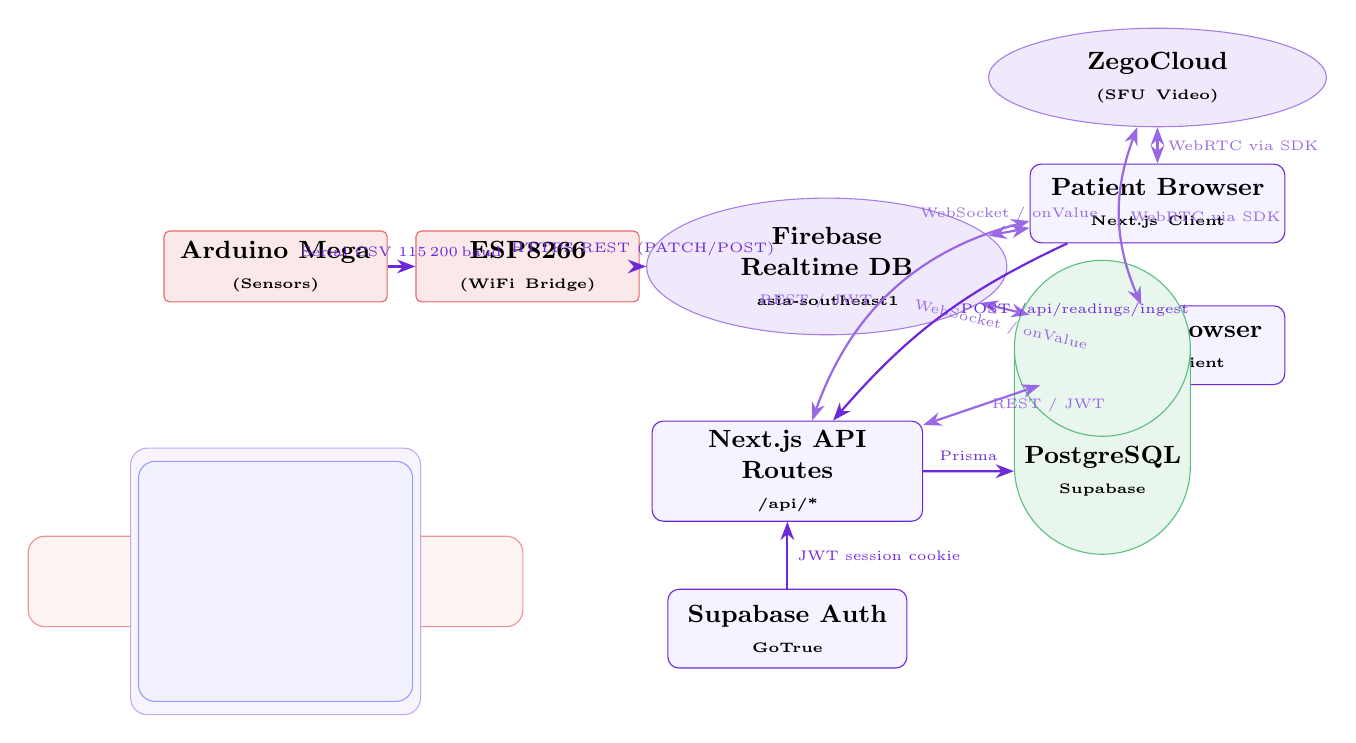
\begin{tikzpicture}

  %─── Hardware tier (top-left) ──────────────────────────────────────────────
  \node[hw, text width=2.6cm] at (0, 4)     (arduino) {Arduino Mega\\{\tiny (Sensors)}};
  \node[hw, text width=2.6cm] at (3.2, 4)   (esp)     {ESP8266\\{\tiny (WiFi Bridge)}};

  %─── Firebase (top-centre) ─────────────────────────────────────────────────
  \node[cloud, text width=3.0cm] at (7, 4)  (fb)      {Firebase\\Realtime DB\\{\tiny asia-southeast1}};

  %─── Browser clients (right) ───────────────────────────────────────────────
  \node[block=3.0cm] at (11.2, 4.8)         (patient) {Patient Browser\\{\tiny Next.js Client}};
  \node[block=3.0cm] at (11.2, 3.0)         (doctor)  {Doctor Browser\\{\tiny Next.js Client}};

  %─── ZegoCloud (top-right) ─────────────────────────────────────────────────
  \node[cloud, text width=2.8cm] at (11.2, 6.4) (zego) {ZegoCloud\\{\tiny (SFU Video)}};

  %─── Next.js API (centre-bottom) ───────────────────────────────────────────
  \node[block=3.2cm] at (6.5, 1.4)          (api)     {Next.js API Routes\\{\tiny /api/*}};

  %─── PostgreSQL (right of API) ─────────────────────────────────────────────
  \node[db] at (10.5, 1.4)                   (pg)      {PostgreSQL\\{\tiny Supabase}};

  %─── Supabase Auth (below API) ─────────────────────────────────────────────
  \node[block=2.8cm] at (6.5, -0.6)         (auth)    {Supabase Auth\\{\tiny GoTrue}};

  %─── Edges ─────────────────────────────────────────────────────────────────
  % Hardware chain
  \draw[arrow] (arduino) -- node[above, font=\tiny] {Serial CSV 115\,200\,baud} (esp);

  % ESP8266 → Firebase (primary real-time upload)
  \draw[arrow] (esp) -- node[above, font=\tiny] {HTTPS REST (PATCH/POST)} (fb);

  % Firebase ↔ Patient Browser (WebSocket subscription)
  \draw[darrow] (fb) -- node[above, font=\tiny] {WebSocket / onValue} (patient);

  % Firebase ↔ Doctor Browser
  \draw[darrow] (fb) -- node[below, font=\tiny, sloped] {WebSocket / onValue} (doctor);

  % Patient Browser → API: ingest readings into PostgreSQL
  \draw[arrow, bend right=12] (patient) to
        node[right, font=\tiny, pos=0.45] {POST /api/readings/ingest} (api);

  % Patient Browser ↔ API: general REST
  \draw[darrow, bend right=28] (patient) to
        node[left,  font=\tiny, pos=0.55] {REST / JWT} (api);

  % Doctor Browser ↔ API: REST only
  \draw[darrow] (doctor) -- node[right, font=\tiny] {REST / JWT} (api);

  % API → PostgreSQL
  \draw[arrow] (api) -- node[above, font=\tiny] {Prisma} (pg);

  % Auth → API (JWT session cookie)
  \draw[arrow] (auth) -- node[right, font=\tiny] {JWT session cookie} (api);

  % Browsers ↔ ZegoCloud (1-on-1 video)
  \draw[darrow] (patient) -- node[right, font=\tiny] {WebRTC via SDK} (zego);
  \draw[darrow] (doctor)  to[bend left=22]
        node[right, font=\tiny] {WebRTC via SDK} (zego);

  %─── Background zones ──────────────────────────────────────────────────────
  \begin{pgfonlayer}{background}
    \node[draw=codered!50, fill=codered!5, rounded corners=6pt,
          fit=(arduino)(esp),
          label={[font=\tiny\bfseries\color{codered}]above:Hardware Tier}] {};
    \node[draw=accent!40, fill=accent!5, rounded corners=6pt,
          fit=(api)(auth),
          label={[font=\tiny\bfseries\color{accent}]below:App Server Tier}] {};
    \node[draw=blue!40, fill=blue!5, rounded corners=6pt,
          fit=(patient)(doctor),
          label={[font=\tiny\bfseries\color{blue!70!black}]right:Client Tier}] {};
  \end{pgfonlayer}

\end{tikzpicture}%
}
\caption{MindMonitor high-level component diagram. Arduino Mega and ESP8266
are separate chips; ESP8266 writes directly to Firebase RTDB via HTTPS REST.
Double-headed arrows indicate bidirectional data flow.}
\label{fig:arch}
\end{figure}

\section{Scaling Boundaries and Failure Domains}

\begin{description}[leftmargin=0em]
  \item[Stateless API tier] Next.js API routes carry no in-process
    state; every request independently opens a Prisma connection from
    the PgBouncer pool. Horizontal scaling (multiple Next.js instances)
    requires no coordination.

  \item[Firebase as shared bus] All ESP8266 devices and all connected
    browsers share the same RTDB tree, partitioned only by session
    identifier. Firebase's managed infrastructure handles fan-out.
    A Firebase outage degrades live dashboards but does not corrupt
    PostgreSQL history.

  \item[PostgreSQL connection pool] PgBouncer in transaction mode
    (\texttt{pgbouncer=true}) limits the effective connection count
    presented to Postgres, preventing connection exhaustion under
    serverless function concurrency. Prisma migrations use the
    direct URL to bypass the pooler.

  \item[Hardware resilience] The ESP8266 polls \texttt{/bridge/activeSession}
    before each upload cycle. If the RTDB write fails (HTTP non-2xx),
    the current reading cycle is silently dropped; the Arduino continues
    sampling and the next cycle retries independently.

  \item[Fallback / demo mode] When no active Firebase session exists,
    \texttt{useSessionStream} and the SSE endpoint
    \texttt{/api/sessions/[id]/stream} emit synthetically generated
    readings via \texttt{src/lib/fakeReading.ts}, ensuring the
    dashboards remain demonstrable without hardware.
\end{description}

% ═══════════════════════════════════════════════════════════════════════════
\chapter{Core Technical Workflows}
\label{ch:workflows}

\section{Authentication \& Session Management}
\label{sec:auth}

\subsection{Architecture Role and Trigger Points}

Authentication is enforced at two independent layers: the Edge middleware
(\texttt{src/middleware.ts}) rejects or redirects unauthenticated HTTP
requests before any page or API handler executes, and each sensitive
API route independently verifies the Supabase session to obtain the
caller's \texttt{userId} and \texttt{role}.

\subsection{Registration Flow}

\begin{enumerate}[leftmargin=1.5em, itemsep=0.2em]
  \item The client submits \texttt{email}, \texttt{password}, \texttt{name},
        and \texttt{role} (\texttt{PATIENT} or \texttt{DOCTOR}) to
        \texttt{POST /api/auth/register}.
  \item The route calls \texttt{supabase.auth.signUp()} via the admin
        client (service-role key), embedding \texttt{role} and
        \texttt{name} in Supabase's \texttt{user\_metadata}.
  \item A corresponding \texttt{User} record is created in PostgreSQL
        via Prisma with the same \texttt{id} as the Supabase UID,
        ensuring referential integrity across both stores.
  \item Auto-assignment: if the new user is a \texttt{PATIENT}, the
        route queries all existing \texttt{DOCTOR} users and inserts
        a \texttt{PatientDoctor} row for each pair. Conversely, a new
        \texttt{DOCTOR} is assigned all existing patients. This simplifies
        the MVP by eliminating a separate assignment step.
  \item The route optionally calls \texttt{/api/auth/confirm-email}
        (which invokes \texttt{supabase.auth.admin.updateUser} with
        \texttt{email\_confirm: true}) to bypass the email verification
        gate in development.
\end{enumerate}

\subsection{Login Flow}

\begin{enumerate}[leftmargin=1.5em, itemsep=0.2em]
  \item Client calls \texttt{supabase.auth.signInWithPassword()}.
  \item On \texttt{email\_not\_confirmed} error, an automatic confirmation
        call is made and sign-in is retried.
  \item On success, Supabase writes an \texttt{sb-<project>-auth-token}
        cookie.
  \item The client reads \texttt{user.user\_metadata.role} and navigates
        to \texttt{/doctor/dashboard} or \texttt{/patient/dashboard}.
\end{enumerate}

\subsection{Middleware Route Guard}

The middleware matcher excludes \texttt{/api/sensor} (hardware endpoint
authenticated via \texttt{x-api-key} header) and Next.js internals.
For all other matched paths it:

\begin{enumerate}[leftmargin=1.5em, itemsep=0.2em]
  \item Calls \texttt{supabase.auth.getUser()} using the SSR-compatible
        client (reads cookie from request headers).
  \item If unauthenticated and path requires auth $\to$ redirect to \texttt{/login}.
  \item If authenticated and path is \texttt{/login} or \texttt{/register}
        $\to$ redirect to role-appropriate dashboard.
  \item Enforces cross-role access: a \texttt{PATIENT} hitting
        \texttt{/doctor/dashboard} is redirected; a \texttt{DOCTOR}
        hitting \texttt{/patient/dashboard} is redirected.
  \item Unknown roles (e.g., \texttt{ADMIN}) are passed through without
        redirection to avoid loops. [Verify in \texttt{src/middleware.ts}]
\end{enumerate}

\subsection{Security Considerations}

\begin{itemize}[leftmargin=1.5em]
  \item The hardware endpoint \texttt{POST /api/sensor} compares the
        \texttt{x-api-key} header against the \texttt{ARDUINO\_API\_KEY}
        environment variable, providing a lightweight secret-based
        authentication separate from user sessions.
  \item The service-role key (\texttt{SUPABASE\_SERVICE\_ROLE\_KEY}) is
        never exposed to the client; it is used only in server-only
        Supabase admin calls.
  \item ZegoCloud tokens are generated server-side using HMAC-SHA256
        over \texttt{APP\_ID + ROOM\_ID + USER\_ID + expiration}.
        [Assumption: token generation occurs within \texttt{VideoCallRoom.tsx}
        or an adjacent server action; verify exact token endpoint.]
\end{itemize}

% ────────────────────────────────────────────────────────────────────────────
\section{Server-Side Rendering (SSR) Pipeline}
\label{sec:ssr}

\subsection{Architecture Role}

Next.js App Router combines React Server Components (RSC) for
data-fetching shells with Client Components for interactive widgets.
The SSR pipeline executes per request for dynamic routes and is
revalidated on-demand for cacheable data.

\subsection{Data Flow}

\begin{enumerate}[leftmargin=1.5em, itemsep=0.2em]
  \item Browser issues a navigation request (e.g., \texttt{GET /doctor/dashboard}).
  \item Edge Middleware validates the Supabase session cookie; if valid,
        the request proceeds to the RSC renderer.
  \item The Server Component may call internal API routes or Prisma
        directly to hydrate initial page data (patient list, recent
        alerts). [Assumption: Server Components call Prisma directly
        rather than fetching \texttt{/api/*} routes; verify in page files.]
  \item React serialises the RSC payload and streams HTML to the browser.
  \item Client Components (\texttt{"use client"} directive) hydrate in
        the browser; \texttt{useEffect} hooks fire to attach Firebase
        listeners and start live-data subscriptions.
  \item Subsequent interactions travel as standard \texttt{fetch} calls
        to \texttt{/api/*} routes without full page reloads.
\end{enumerate}

\subsection{Route Groups and Layouts}

Route groups (\texttt{(auth)}, \texttt{(patient)}, \texttt{(doctor)})
provide layout isolation: each group can define its own
\texttt{layout.tsx} with role-specific navigation, sidebar components,
and data-fetching context without leaking into sibling groups.

% ────────────────────────────────────────────────────────────────────────────
\section{ESP8266 $\leftrightarrow$ Firebase Realtime Database Bridge}
\label{sec:bridge}

\subsection{Architecture Role}

The ESP8266 acts as the network gateway for the sensor node. It
maintains a persistent WiFi connection and translates the Arduino's
synchronous serial output into asynchronous Firebase REST writes.

\subsection{Step-by-Step Data Flow}

\begin{enumerate}[leftmargin=1.5em, itemsep=0.2em]
  \item \textbf{Serial receive}: ESP8266 listens on the hardware serial
        port at 9600 baud. When a complete line arrives from the Arduino,
        it is buffered and parsed into named fields:
        \texttt{temperature}, \texttt{gsrRaw}, \texttt{heartRate},
        \texttt{spo2}, \texttt{stressScore}, \texttt{stressLabel},
        \texttt{ir}, \texttt{red}, \texttt{fingerDetected},
        \texttt{skinDetected}, \texttt{gsrBaseline}, \texttt{gsrDiff},
        \texttt{status}.

  \item \textbf{Session lookup}: The ESP8266 issues an HTTPS GET to
        the Firebase RTDB at \texttt{/bridge/activeSession.json}.
        The response JSON contains \texttt{sessionId} and
        \texttt{patientId}. If no active session is found, the upload
        cycle is skipped.

  \item \textbf{Current-state write}: An HTTPS PATCH request merges
        the latest reading into \texttt{/live/current/\{sessionId\}.json},
        overwriting the previous value. Any browser subscribed to this
        path receives an immediate push notification from Firebase.

  \item \textbf{History append}: An HTTPS POST to
        \texttt{/history/readings/\{sessionId\}.json} appends a new
        child node with a server-generated push key. A
        \texttt{timeStampMs} field (milliseconds since epoch, from
        \texttt{millis()}) is included for ordering and deduplication.

  \item The ESP8266 waits approximately 1.5 seconds before the next
        cycle, synchronised with the Arduino's output cadence.
\end{enumerate}

\subsection{Arduino Sensor Logic}

The Arduino Mega samples sensors on each loop iteration:

\begin{itemize}[leftmargin=1.5em]
  \item \textbf{MAX30102}: Reads IR and red LED values over I2C.
        BPM is derived from the inter-beat interval (IBI) computed
        by tracking peaks in the IR waveform. SpO2 is approximated
        from the ratio $R = \ln(\text{red})/\ln(\text{IR})$ using a
        lookup table.
  \item \textbf{DS18B20}: Temperature is read via OneWire on digital
        pin 3.
  \item \textbf{GSR}: Raw ADC value from A1 scaled to a 0--100 index
        with a rolling 10-sample baseline.
  \item \textbf{Stress score}: A composite 0--4 integer derived from:
        GSR $>$ threshold, temperature outside 36.0--37.8~\textdegree{}C,
        BPM outside 60--90, SpO2 $<$ 95. Each contributing factor
        increments the score by 1.
\end{itemize}

% ────────────────────────────────────────────────────────────────────────────
\section{Video Call System}
\label{sec:video}

\subsection{Architecture Role}

Video consultations connect a doctor and their assigned patient in a
private 1-on-1 call. Room lifecycle is managed by the PostgreSQL
\texttt{VideoAppointment} table; media routing is entirely delegated
to ZegoCloud's Selective Forwarding Unit (SFU) infrastructure.

\subsection{Appointment Lifecycle}

\begin{enumerate}[leftmargin=1.5em, itemsep=0.2em]
  \item \textbf{Scheduling}: Doctor or patient creates an appointment
        via \texttt{POST /api/appointments} supplying
        \texttt{patientId}, \texttt{doctorId}, \texttt{roomId}
        (UUID generated client-side), and \texttt{scheduledAt}.
        Status is set to \texttt{SCHEDULED}.

  \item \textbf{Activation}: Either party patches
        \texttt{/api/appointments/[id]} to status \texttt{ACTIVE},
        which also records \texttt{startedAt = now()}.

  \item \textbf{Room join}: The \texttt{VideoCallRoom.tsx} component
        is rendered when status is \texttt{ACTIVE}. It calls
        \texttt{ZegoUIKitPrebuilt.generateKitTokenForTest()} with:
        \begin{itemize}
          \item \texttt{appID}: \texttt{NEXT\_PUBLIC\_ZEGO\_APP\_ID}
          \item \texttt{serverSecret}: \texttt{NEXT\_PUBLIC\_ZEGO\_SERVER\_SECRET}
          \item \texttt{roomID}: value from \texttt{VideoAppointment.roomId}
          \item \texttt{userID}: Supabase UID of the current user
          \item \texttt{userName}: display name from user metadata
        \end{itemize}
        The token is passed to \texttt{zp.joinRoom()} which initiates
        ICE negotiation with ZegoCloud's TURN/STUN servers.

  \item \textbf{Teardown}: On \texttt{onLeaveRoom} callback, the client
        patches the appointment to \texttt{COMPLETED} and records
        \texttt{endedAt}. [Assumption: no automatic timeout cleanup
        is implemented; verify in \texttt{src/app/api/appointments/[id]/route.ts}]
\end{enumerate}

\subsection{Media Routing and Latency}

ZegoCloud routes media through its SFU network. The client SDK
handles ICE candidate gathering, codec negotiation (VP8/H.264),
and adaptive bitrate. The application has no visibility into media
plane details; the ZegoCloud UIKit component abstracts the WebRTC
\texttt{RTCPeerConnection} lifecycle entirely.

\subsection{Security Considerations}

Token generation uses \texttt{generateKitTokenForTest}, which is
designed for development environments. A production deployment
should move token generation to a server-side endpoint using the
ZegoCloud Server SDK to prevent exposure of \texttt{serverSecret}
in the browser bundle.
[Verify: \texttt{NEXT\_PUBLIC\_ZEGO\_SERVER\_SECRET} is currently
client-exposed; this should be remediated before production.]

% ────────────────────────────────────────────────────────────────────────────
\section{Doctor Evaluation Workflow}
\label{sec:eval}

\subsection{Architecture Role}

Clinical evaluations represent the doctor's structured clinical
assessment of a patient at a point in time. They are persistent,
immutable records in PostgreSQL linking a doctor, patient, and a
set of clinical fields.

\subsection{State Machine}

\begin{center}
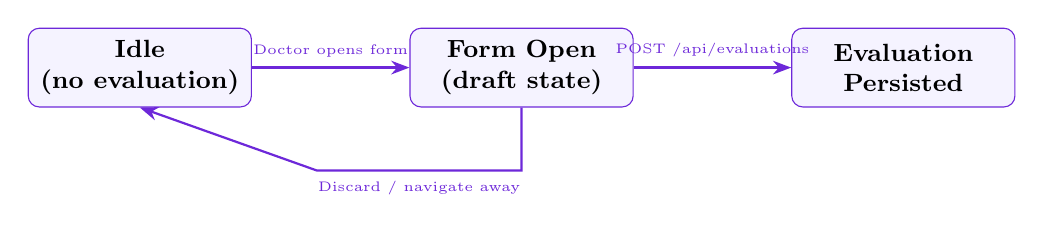
\begin{tikzpicture}[node distance=2.5cm, auto]
  \node[block=2.6cm] (idle) {Idle\\(no evaluation)};
  \node[block=2.6cm, right=2.0cm of idle] (draft) {Form Open\\(draft state)};
  \node[block=2.6cm, right=2.0cm of draft] (submitted) {Evaluation\\Persisted};

  \draw[arrow] (idle) -- node[above, font=\tiny] {Doctor opens form} (draft);
  \draw[arrow] (draft) -- node[above, font=\tiny] {POST /api/evaluations} (submitted);
  \draw[arrow] (draft.south) -- ++(0,-0.8) -- node[below, font=\tiny]
    {Discard / navigate away} ++(-2.6,0) -- (idle.south);
\end{tikzpicture}
\end{center}

\subsection{Step-by-Step Flow}

\begin{enumerate}[leftmargin=1.5em, itemsep=0.2em]
  \item Doctor navigates to a patient's detail page
        (\texttt{/doctor/dashboard/patients/[id]}), triggering the
        \texttt{EvaluationForm.tsx} component to mount.

  \item The form collects: \texttt{diagnosis} (free text),
        \texttt{notes}, \texttt{recommendations}, and
        \texttt{followUpDate} (optional ISO date).

  \item On submit, the client issues \texttt{POST /api/evaluations}
        with \texttt{patientId}, \texttt{doctorId} (from session),
        and the form fields.

  \item The API route validates the payload (Zod), then calls
        \texttt{prisma.evaluation.create()}.

  \item The UI re-fetches \texttt{GET /api/evaluations?patientId=\{id\}}
        to refresh the evaluation history panel, sorted by
        \texttt{createdAt} descending.
\end{enumerate}

\subsection{Data Persistence}

Evaluations are write-once in the current schema (no \texttt{updatedAt}
field, no soft-delete flag). Amendments require creating a new
evaluation record. [Assumption: no audit trail or versioning beyond
\texttt{createdAt} is implemented.]

% ────────────────────────────────────────────────────────────────────────────
\section{Realtime Data Ingestion to PostgreSQL}
\label{sec:ingest}

\subsection{Ingestion Paths}

There are two ingestion paths into the \texttt{SensorReading} table:

\paragraph{Path A --- Firebase Mirror (primary live path)}
The \texttt{useSessionStream} hook in the browser subscribes to Firebase
\texttt{/live/current/\{sessionId\}} and \texttt{/history/readings/\{sessionId\}}.
On each incremental event it calls \texttt{POST /api/readings/ingest}
with the raw Firebase reading payload. The API route calls
\texttt{ingestFirebaseReadingForPatient()} from
\texttt{src/lib/firebaseReadingsSync.ts}, which:

\begin{enumerate}[leftmargin=1.5em, itemsep=0.1em]
  \item Normalises field names (handles \texttt{timeStampMs}/\texttt{timestampMs}
        variant spellings).
  \item Converts the timestamp to a \texttt{Date} object (\texttt{recordedAt}).
  \item Calls \texttt{prisma.sensorReading.upsert()} using
        \texttt{sourceTimestampMs} as the unique conflict key,
        preventing duplicate rows when the hook fires multiple times
        for the same reading.
\end{enumerate}

After ingestion, the route executes \texttt{checkAnomaly()} from
\texttt{src/lib/anomaly.ts}. If a threshold is breached, a new
\texttt{Alert} record is created via Prisma, immediately visible to
both the patient and doctor.

\paragraph{Path B --- Hardware Serial Bridge}
The \texttt{bridge/} directory contains a Node.js script that reads from
the system serial port using \texttt{serialport} v13 and calls
\texttt{POST /api/sensor} with an \texttt{x-api-key} header.
[Verify bridge entry point in \texttt{bridge/} directory.]

\paragraph{Path C --- SSE Fake Stream (demo mode)}
\texttt{GET /api/sessions/[id]/stream} returns a Server-Sent Events
response. The handler calls \texttt{nextReading()} from
\texttt{src/lib/fakeReading.ts} every 1500~ms using
\texttt{setInterval}. This path does not write to PostgreSQL; it is
consumed by \texttt{useLiveSession.ts} in dummy mode.

\subsection{Anomaly Detection}

\texttt{src/lib/anomaly.ts} implements two entry points:

\begin{itemize}[leftmargin=1.5em]
  \item \texttt{checkAnomaly(reading, patientId)} --- async; queries the
        last $N$ readings for the patient to detect \textbf{prolonged stress}
        (5 or more consecutive readings with \texttt{stressScore} $\geq 3$).
        Also checks single-reading thresholds: high stress, temperature
        anomaly (outside 35.5--37.8~\textdegree{}C), and rapid change.

  \item \texttt{detectAnomaly(reading)} --- synchronous; returns a severity
        label and description without database I/O. Used for in-memory
        classification during batch processing.
\end{itemize}

Alert types are typed as the \texttt{AlertType} enum:
\texttt{HIGH\_STRESS}, \texttt{PROLONGED\_STRESS},
\texttt{RAPID\_CHANGE}, \texttt{TEMPERATURE\_ANOMALY}.

% ────────────────────────────────────────────────────────────────────────────
\section{Prisma ORM Integration}
\label{sec:prisma}

\subsection{Client Instantiation}

\texttt{src/lib/prisma.ts} uses the canonical Next.js singleton pattern
to prevent connection pool exhaustion under HMR:

\begin{lstlisting}[language=JavaScript, caption={Prisma singleton pattern}]
const globalForPrisma = globalThis as unknown as { prisma: PrismaClient };
const prisma = globalForPrisma.prisma
  ?? new PrismaClient({ log: ["error"] });
if (process.env.NODE_ENV !== "production")
  globalForPrisma.prisma = prisma;
export default prisma;
\end{lstlisting}

\subsection{Connection Handling}

Two database URLs are configured:

\begin{itemize}[leftmargin=1.5em]
  \item \texttt{DATABASE\_URL}: PgBouncer pooler endpoint on port 6543
        with \texttt{pgbouncer=true}. Used by the application at runtime.
        PgBouncer in transaction mode multiplexes application connections
        onto a limited pool of server connections.

  \item \texttt{DIRECT\_URL}: Direct Postgres endpoint on port 5432.
        Declared as \texttt{directUrl} in \texttt{prisma/schema.prisma}
        for Prisma Migrate, which requires a non-pooled connection to
        execute DDL statements reliably.
\end{itemize}

\subsection{Schema Mapping}

The Prisma schema declares models that map directly to PostgreSQL tables.
All models use \texttt{@default(cuid())} primary keys (CUID v1 strings)
for sortable, URL-safe identifiers without UUID generation overhead.

\subsection{Query Patterns}

\begin{itemize}[leftmargin=1.5em]
  \item \textbf{Range reads}: \texttt{GET /api/readings} accepts
        \texttt{range=24h|7d|30d}, converting to a
        \texttt{where: \{ recordedAt: \{ gte: cutoff \} \}} predicate
        that uses the \texttt{(patientId, recordedAt)} compound index.

  \item \textbf{Upsert with deduplication}: Sensor readings from
        Firebase are upserted on \texttt{sourceTimestampMs} to avoid
        duplicate rows when the client hook fires multiple times.

  \item \textbf{Enriched patient list}: \texttt{GET /api/patients} joins
        \texttt{PatientDoctor}, selects the latest reading per patient,
        and counts unread alerts in a single Prisma query using
        \texttt{include} and \texttt{\_count} aggregations.

  \item \textbf{Transactions}: The registration flow wraps
        \texttt{prisma.user.create()} and
        \texttt{prisma.patientDoctor.createMany()} in a Prisma
        interactive transaction to ensure atomicity of the user +
        assignment pair. [Verify in \texttt{src/app/api/auth/register/route.ts}]
\end{itemize}

% ────────────────────────────────────────────────────────────────────────────
\section{Firebase Realtime Sync Mechanism}
\label{sec:firebase}

\subsection{RTDB Tree Structure}

\begin{lstlisting}[caption={Firebase RTDB path schema}]
/bridge/
  activeSession/
    sessionId: "<cuid>"
    patientId: "<cuid>"

/live/
  current/
    {sessionId}/      <- PATCH on each ESP8266 cycle
      temperature, gsrRaw, heartRate, spo2,
      stressScore, timeStampMs, ...

/history/
  readings/
    {sessionId}/
      {pushKey}/      <- POST appended by ESP8266
        <same fields as live/current>
\end{lstlisting}

\subsection{Browser Listeners}

\texttt{src/hooks/useSessionStream.ts} attaches two Firebase listeners
on component mount:

\begin{enumerate}[leftmargin=1.5em, itemsep=0.2em]
  \item \texttt{onValue(ref(db, "live/current/"+sessionId), ...)}: fires
        on every PATCH from the ESP8266, updating the \texttt{reading}
        state used by the live vitals panel.

  \item \texttt{onChildAdded(ref(db, "history/readings/"+sessionId), ...)}:
        fires for each new push key added to the history tree, providing
        the ordered stream consumed by time-series charts and the
        PostgreSQL ingestion pipeline.
\end{enumerate}

Listeners are detached on component unmount via the returned unsubscribe
function to prevent memory leaks.

\subsection{Offline Cache and Conflict Resolution}

The Firebase Web SDK v9+ enables disk persistence on supported browsers
by default. [Assumption: \texttt{enablePersistence()} is not explicitly
called; verify in \texttt{src/lib/firebase.ts}.] Without explicit
persistence, the SDK uses an in-memory cache only. On reconnect,
Firebase re-delivers any missed events since the last listener
timestamp; the \texttt{onChildAdded} listener's deduplication logic
(based on \texttt{sourceTimestampMs} and a content hash) prevents
duplicate PostgreSQL rows from missed-event replays.

\subsection{Server-Side RTDB Operations}

\texttt{src/lib/firebaseRtdbServer.ts} provides typed wrappers
(\texttt{rtdbGet}, \texttt{rtdbPut}, \texttt{rtdbPatch}, \texttt{rtdbPost},
\texttt{rtdbDelete}) that call the Firebase REST API via \texttt{fetch}.
These are used in API routes to write session data (e.g., publishing
\texttt{/bridge/activeSession} when a new monitoring session is created)
without bundling the Firebase client SDK into the server bundle.

% ────────────────────────────────────────────────────────────────────────────
\section{Routing \& Navigation}
\label{sec:routing}

\subsection{Route Structure}

\begin{longtable}{L{5.5cm} L{2.5cm} L{6.5cm}}
  \caption{Application Routes\label{tab:routes}} \\
  \toprule
  \textbf{Path} & \textbf{Type} & \textbf{Description} \\
  \midrule
  \endfirsthead
  \multicolumn{3}{c}{\textit{continued}} \\ \midrule
  \endhead
  \bottomrule
  \endfoot

  \texttt{/} & Public & Landing page (Hero, Features, CTA) \\
  \rowcolor{rowalt}
  \texttt{/login} & Auth-only & Email/password sign-in with role redirect \\
  \texttt{/register} & Auth-only & New user registration \\
  \rowcolor{rowalt}
  \texttt{/patient/dashboard} & Patient & Live vitals, session controls, history \\
  \texttt{/patient/dashboard/evaluations} & Patient & View doctor evaluations \\
  \rowcolor{rowalt}
  \texttt{/patient/dashboard/history} & Patient & Historical sensor data table \\
  \texttt{/doctor/dashboard} & Doctor & Patient list, alerts feed \\
  \rowcolor{rowalt}
  \texttt{/doctor/dashboard/patients/[id]} & Doctor & Patient detail, live data, evaluation form \\
  \texttt{/doctor/dashboard/evaluate} & Doctor & Standalone evaluation form \\
\end{longtable}

\subsection{Dynamic Routes}

\texttt{/doctor/dashboard/patients/[id]} uses Next.js dynamic segment
routing. The \texttt{id} parameter is the Prisma \texttt{User.id} (CUID).
The page component receives \texttt{params.id} as a prop and passes it
to \texttt{GET /api/patients} and related API calls.

\subsection{Middleware Guards}

The middleware matcher pattern matches
\texttt{/(doctor|patient)/dashboard(.*)} and \texttt{/dashboard}.
The \texttt{/api/sensor} path is explicitly excluded to allow the
hardware bridge to post without session cookies.

\subsection{SSR Hydration}

For dashboard pages, the Server Component shell fetches initial data
(e.g., patient list) during SSR, serialises it into the RSC payload,
and streams it to the browser. The Client Component receives this as
\texttt{initialData} props and uses it to render the first frame
without a loading spinner, then transitions to live Firebase data
as \texttt{useEffect} hooks fire during hydration.
[Assumption: initial props pattern used; verify in dashboard page.tsx files.]

% ═══════════════════════════════════════════════════════════════════════════
\chapter{Database Schema \& ER Diagram}
\label{ch:db}

\section{Prisma Schema Overview}

The PostgreSQL schema comprises seven primary models. All primary keys
are CUID strings. Foreign keys enforce referential integrity at the
database level via Prisma's \texttt{@relation} directive, which emits
\texttt{FOREIGN KEY ... ON DELETE CASCADE} or \texttt{RESTRICT} clauses
depending on the relation type.

\section{Model Definitions}

\subsection{User}

\begin{longtable}{L{3.5cm} L{2.8cm} L{2.0cm} L{5.5cm}}
  \caption{User model fields\label{tab:user}} \\
  \toprule
  \textbf{Field} & \textbf{Prisma Type} & \textbf{Nullable} & \textbf{Notes} \\
  \midrule
  \endfirsthead \multicolumn{4}{c}{\textit{continued}} \\ \midrule \endhead
  \bottomrule \endfoot

  \texttt{id}           & \texttt{String}    & No  & CUID, \texttt{@id} \\
  \rowcolor{rowalt}
  \texttt{email}        & \texttt{String}    & No  & \texttt{@unique}, matches Supabase UID \\
  \texttt{name}         & \texttt{String}    & No  & Display name from registration \\
  \rowcolor{rowalt}
  \texttt{role}         & \texttt{Role} enum & No  & \texttt{PATIENT | DOCTOR | ADMIN} \\
  \texttt{createdAt}    & \texttt{DateTime}  & No  & \texttt{@default(now())} \\
  \rowcolor{rowalt}
  \texttt{readings}     & Relation           & --  & \texttt{SensorReading[]} \\
  \texttt{alerts}       & Relation           & --  & \texttt{Alert[]} (as patient) \\
  \rowcolor{rowalt}
  \texttt{evaluationsAsPatient} & Relation   & --  & \texttt{Evaluation[]} \\
  \texttt{evaluationsAsDoctor}  & Relation   & --  & \texttt{Evaluation[]} \\
  \rowcolor{rowalt}
  \texttt{doctorAssignments}    & Relation   & --  & \texttt{PatientDoctor[]} (as patient) \\
  \texttt{patientAssignments}   & Relation   & --  & \texttt{PatientDoctor[]} (as doctor) \\
  \rowcolor{rowalt}
  \texttt{appointmentsAsPatient}& Relation   & --  & \texttt{VideoAppointment[]} \\
  \texttt{appointmentsAsDoctor} & Relation   & --  & \texttt{VideoAppointment[]} \\
  \texttt{sessions}     & Relation           & --  & \texttt{MonitoringSession[]} \\
\end{longtable}

\subsection{SensorReading}

\begin{longtable}{L{3.5cm} L{2.8cm} L{2.0cm} L{5.5cm}}
  \caption{SensorReading model fields\label{tab:reading}} \\
  \toprule
  \textbf{Field} & \textbf{Prisma Type} & \textbf{Nullable} & \textbf{Notes} \\
  \midrule
  \endfirsthead \multicolumn{4}{c}{\textit{continued}} \\ \midrule \endhead
  \bottomrule \endfoot

  \texttt{id}               & \texttt{String}   & No  & CUID \\
  \rowcolor{rowalt}
  \texttt{patientId}        & \texttt{String}   & No  & FK $\to$ \texttt{User.id} \\
  \texttt{sessionId}        & \texttt{String}   & Yes & FK $\to$ \texttt{MonitoringSession.id} \\
  \rowcolor{rowalt}
  \texttt{deviceId}         & \texttt{String}   & Yes & Hardware serial/identifier \\
  \texttt{temperature}      & \texttt{Float}    & Yes & \textdegree{}C from DS18B20 \\
  \rowcolor{rowalt}
  \texttt{gsrRaw}           & \texttt{Int}      & Yes & Raw ADC value from A1 \\
  \texttt{stressLevel}      & \texttt{Int}      & Yes & Derived 0--4 score \\
  \rowcolor{rowalt}
  \texttt{stressLabel}      & \texttt{String}   & Yes & Human-readable label \\
  \texttt{heartRate}        & \texttt{Float}    & Yes & BPM from MAX30102 \\
  \rowcolor{rowalt}
  \texttt{spo2}             & \texttt{Float}    & Yes & \% SpO2 from MAX30102 \\
  \texttt{gsrBaseline}      & \texttt{Float}    & Yes & Rolling baseline GSR \\
  \rowcolor{rowalt}
  \texttt{gsrDiff}          & \texttt{Float}    & Yes & GSR deviation from baseline \\
  \texttt{ir}               & \texttt{Float}    & Yes & Raw IR photoplethysmographic value \\
  \rowcolor{rowalt}
  \texttt{red}              & \texttt{Float}    & Yes & Raw red LED value \\
  \texttt{fingerDetected}   & \texttt{Boolean}  & Yes & MAX30102 presence flag \\
  \rowcolor{rowalt}
  \texttt{skinDetected}     & \texttt{Boolean}  & Yes & GSR contact flag \\
  \texttt{stressScore}      & \texttt{Float}    & Yes & Normalised 0.0--1.0 score \\
  \rowcolor{rowalt}
  \texttt{status}           & \texttt{String}   & Yes & Reading quality status \\
  \texttt{sourceTimestampMs}& \texttt{BigInt}   & Yes & \texttt{@unique}; millis from hardware \\
  \rowcolor{rowalt}
  \texttt{recordedAt}       & \texttt{DateTime} & No  & \texttt{@default(now())} \\
  \multicolumn{4}{l}{\textit{Indexes}: \texttt{(patientId, recordedAt)},
    \texttt{(sessionId, recordedAt)}} \\
\end{longtable}

\subsection{Alert}

Fields: \texttt{id} (CUID), \texttt{patientId} (FK User), \texttt{type}
(\texttt{AlertType} enum), \texttt{message}, \texttt{severity},
\texttt{acknowledged} (Boolean, default false), \texttt{createdAt}.

\subsection{Evaluation}

Fields: \texttt{id}, \texttt{patientId} (FK User), \texttt{doctorId}
(FK User), \texttt{diagnosis}, \texttt{notes}, \texttt{recommendations},
\texttt{followUpDate} (DateTime, nullable), \texttt{createdAt}.

\subsection{PatientDoctor}

Composite primary key: \texttt{(patientId, doctorId)}. Both fields are
foreign keys to \texttt{User.id}. This join table implements the
many-to-many doctor-patient assignment relationship.

\subsection{MonitoringSession}

Fields: \texttt{id}, \texttt{patientId} (FK User), \texttt{deviceId}
(nullable), \texttt{status} (\texttt{ACTIVE | ENDED}), \texttt{startedAt},
\texttt{endedAt} (nullable). Relation: \texttt{readings SensorReading[]}.

\subsection{VideoAppointment}

Fields: \texttt{id}, \texttt{patientId} (FK User), \texttt{doctorId}
(FK User), \texttt{roomId} (\texttt{@unique}), \texttt{scheduledAt},
\texttt{status} (\texttt{SCHEDULED | ACTIVE | COMPLETED | CANCELLED}),
\texttt{startedAt}, \texttt{endedAt}. Indexes: \texttt{(patientId)},
\texttt{(doctorId)}.

\section{Enumerations}

\begin{itemize}[leftmargin=1.5em]
  \item \texttt{Role}: \texttt{PATIENT}, \texttt{DOCTOR}, \texttt{ADMIN}
  \item \texttt{AlertType}: \texttt{HIGH\_STRESS}, \texttt{PROLONGED\_STRESS},
        \texttt{RAPID\_CHANGE}, \texttt{TEMPERATURE\_ANOMALY}
  \item \texttt{SessionStatus}: \texttt{ACTIVE}, \texttt{ENDED}
  \item \texttt{AppointmentStatus}: \texttt{SCHEDULED}, \texttt{ACTIVE},
        \texttt{COMPLETED}, \texttt{CANCELLED}
\end{itemize}

\section{ER Diagram}

\begin{figure}[h!]
\centering
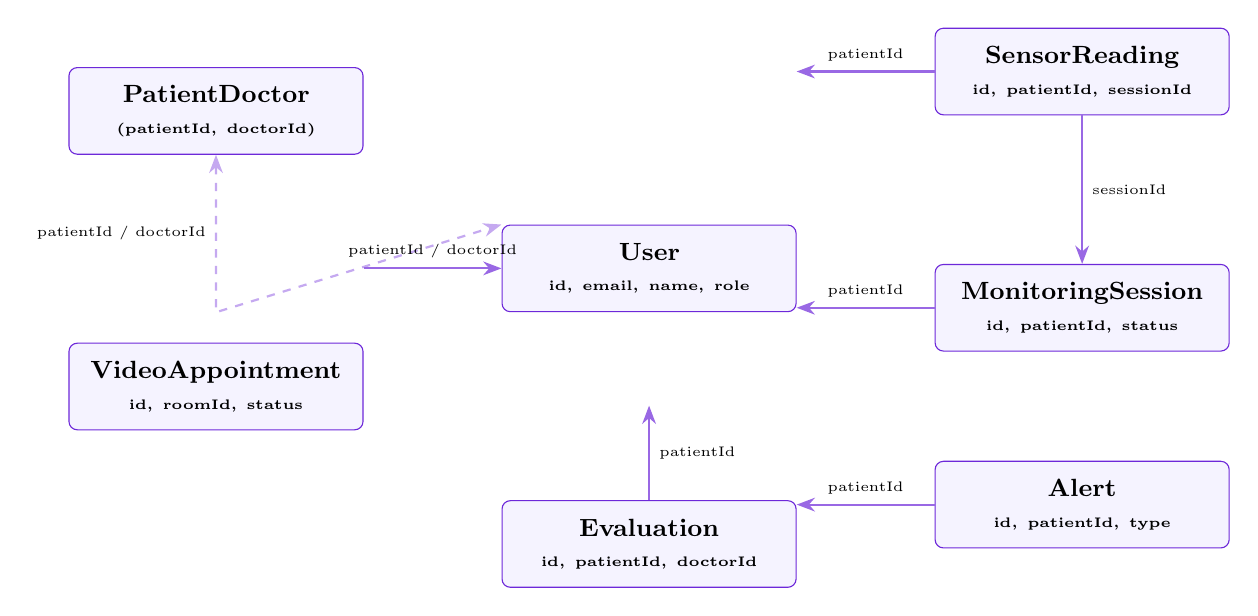
\begin{tikzpicture}[
  entity/.style={rectangle, draw=accent, fill=rowalt, rounded corners=3pt,
                 text width=3.5cm, align=center, minimum height=1.1cm,
                 font=\small\bfseries},
  fk/.style={-Stealth, thick, draw=accent!70},
  m2m/.style={Stealth-Stealth, thick, draw=accent!40, dashed}
]
  \node[entity] (user)    at (0, 0)       {User\\{\tiny id, email, name, role}};
  \node[entity] (reading) at (5.5, 2.5)   {SensorReading\\{\tiny id, patientId, sessionId}};
  \node[entity] (session) at (5.5, -0.5)  {MonitoringSession\\{\tiny id, patientId, status}};
  \node[entity] (alert)   at (5.5, -3.0)  {Alert\\{\tiny id, patientId, type}};
  \node[entity] (eval)    at (0, -3.5)    {Evaluation\\{\tiny id, patientId, doctorId}};
  \node[entity] (appt)    at (-5.5, -1.5) {VideoAppointment\\{\tiny id, roomId, status}};
  \node[entity] (pd)      at (-5.5, 2.0)  {PatientDoctor\\{\tiny (patientId, doctorId)}};

  \draw[fk] (reading.west) -- node[above, font=\tiny] {patientId}
    (user.east |- reading.west);
  \draw[fk] (session.west) -- node[above, font=\tiny] {patientId}
    (user.east |- session.west);
  \draw[fk] (alert.west)   -- node[above, font=\tiny] {patientId}
    (user.east |- alert.west);
  \draw[fk] (reading.south) -- node[right, font=\tiny] {sessionId}
    (session.north);
  \draw[fk] (eval.north)    -- node[right, font=\tiny] {patientId}
    ++(0, 1.2);
  \draw[m2m] (pd.south) -- node[left, font=\tiny] {patientId / doctorId}
    ++(0,-2.0) -- (user.north west);
  \draw[fk] (appt.east |- user) -- node[above, font=\tiny]
    {patientId / doctorId} (user.west);
\end{tikzpicture}
\caption{Simplified Entity-Relationship diagram. Dashed bidirectional
arrow denotes many-to-many resolved via join table.}
\label{fig:er}
\end{figure}

\section{Indexing Strategy}

\begin{itemize}[leftmargin=1.5em]
  \item \textbf{\texttt{(patientId, recordedAt)} on \texttt{SensorReading}}:
        Supports range queries in \texttt{GET /api/readings} with a
        leading equality predicate on \texttt{patientId} and a range
        scan on \texttt{recordedAt}.

  \item \textbf{\texttt{(sessionId, recordedAt)} on \texttt{SensorReading}}:
        Optimises session-scoped history loads used in monitoring panels
        and the SSE stream.

  \item \textbf{\texttt{(patientId)} and \texttt{(doctorId)} on \texttt{VideoAppointment}}:
        Separate single-column indexes support independent lookups by
        either participant role.

  \item \textbf{\texttt{sourceTimestampMs @unique} on \texttt{SensorReading}}:
        Enforces deduplication at the database level and provides a
        unique index used by Prisma's \texttt{upsert} conflict target.

  \item \textbf{\texttt{roomId @unique} on \texttt{VideoAppointment}}:
        Prevents duplicate room creation; used as a natural lookup key
        when joining a ZegoCloud room.

  \item \textbf{\texttt{email @unique} on \texttt{User}}:
        Standard uniqueness constraint mirroring Supabase Auth's email
        uniqueness.
\end{itemize}

% ═══════════════════════════════════════════════════════════════════════════
\chapter{Security Overview}
\label{ch:security}

\section{Authentication Boundaries}

\begin{description}[leftmargin=0em, itemsep=0.4em]
  \item[Browser $\to$ API]
    All authenticated API routes rely on the Supabase JWT stored in
    an HTTP-only session cookie. The middleware verifies the token
    signature before page rendering. API routes that require a user
    identity call \texttt{supabase.auth.getUser()} from the request
    context.

  \item[Hardware $\to$ API]
    \texttt{POST /api/sensor} is excluded from cookie-based auth.
    Instead it requires the \texttt{x-api-key} header to match
    \texttt{process.env.ARDUINO\_API\_KEY}. This key should be rotated
    periodically and stored securely on the ESP8266 firmware.

  \item[ESP8266 $\to$ Firebase]
    The ESP8266 uses Firebase's legacy REST auth model. A Firebase
    Database Security Rule should restrict write access to authenticated
    clients or specific API keys.
    [Verify: Firebase rules may currently allow open writes ---
    this must be hardened before production deployment.]

  \item[Server $\to$ Supabase Admin]
    The service-role key is stored in \texttt{SUPABASE\_SERVICE\_ROLE\_KEY}
    (server-only environment variable, no \texttt{NEXT\_PUBLIC\_} prefix).
    It is never included in the client bundle.
\end{description}

\section{Known Security Risks}

\begin{enumerate}[leftmargin=1.5em]
  \item \texttt{NEXT\_PUBLIC\_ZEGO\_SERVER\_SECRET} is client-exposed
        (the \texttt{NEXT\_PUBLIC\_} prefix makes it visible in the
        browser bundle). Token generation should be moved to a server
        action.

  \item WiFi credentials (SSID and password) are hardcoded in the
        ESP8266 firmware. In a production deployment these should be
        provisioned via WiFi Manager or a secure OTA mechanism.

  \item Firebase RTDB security rules are not shown in the codebase.
        Without explicit rules, the database may be open to
        unauthenticated reads or writes.
\end{enumerate}

% ═══════════════════════════════════════════════════════════════════════════
\chapter{Deployment \& Environment Configuration}
\label{ch:deploy}

\section{Environment Variables}

\begin{longtable}{L{6.5cm} L{8.0cm}}
  \caption{Required environment variables\label{tab:env}} \\
  \toprule
  \textbf{Variable} & \textbf{Purpose} \\
  \midrule
  \endfirsthead \multicolumn{2}{c}{\textit{continued}} \\ \midrule \endhead
  \bottomrule \endfoot

  \texttt{DATABASE\_URL} & Prisma runtime connection (PgBouncer, port 6543) \\
  \rowcolor{rowalt}
  \texttt{DIRECT\_URL}   & Prisma Migrate connection (direct, port 5432) \\
  \texttt{NEXT\_PUBLIC\_SUPABASE\_URL}  & Supabase project URL \\
  \rowcolor{rowalt}
  \texttt{NEXT\_PUBLIC\_SUPABASE\_ANON\_KEY} & Public anon key \\
  \texttt{SUPABASE\_SERVICE\_ROLE\_KEY} & Admin key (server-only) \\
  \rowcolor{rowalt}
  \texttt{ARDUINO\_API\_KEY} & Hardware endpoint secret \\
  \texttt{NEXT\_PUBLIC\_ZEGO\_APP\_ID} & ZegoCloud application ID \\
  \rowcolor{rowalt}
  \texttt{NEXT\_PUBLIC\_ZEGO\_SERVER\_SECRET} & ZegoCloud secret (should be server-only) \\
\end{longtable}

\section{Build and Run}

\begin{lstlisting}[caption={Development and production commands}]
# Install dependencies
npm install

# Generate Prisma client
npx prisma generate

# Run Prisma migrations (uses DIRECT_URL)
npx prisma migrate deploy

# Development server
npm run dev

# Production build
npm run build && npm start

# Hardware bridge (desktop serial mode)
node bridge/index.js   # [Verify exact entry point]
\end{lstlisting}

% ═══════════════════════════════════════════════════════════════════════════
\chapter{Appendix: API Route Reference}
\label{ch:api}

\begin{longtable}{L{1.5cm} L{5.5cm} L{7.5cm}}
  \caption{Complete API route inventory\label{tab:api}} \\
  \toprule
  \textbf{Method} & \textbf{Path} & \textbf{Description} \\
  \midrule
  \endfirsthead \multicolumn{3}{c}{\textit{continued}} \\ \midrule \endhead
  \bottomrule \endfoot

  POST  & \texttt{/api/auth/register}           & Create Supabase + Prisma user \\
  \rowcolor{rowalt}
  POST  & \texttt{/api/auth/confirm-email}       & Admin email confirmation bypass \\
  POST  & \texttt{/api/sensor}                   & Hardware reading ingestion (x-api-key) \\
  \rowcolor{rowalt}
  POST  & \texttt{/api/readings/ingest}          & Firebase reading $\to$ PostgreSQL mirror \\
  GET   & \texttt{/api/readings}                 & Paginated reading history by patient+range \\
  \rowcolor{rowalt}
  GET   & \texttt{/api/sessions}                 & Get active session for patient \\
  POST  & \texttt{/api/sessions}                 & Create monitoring session \\
  \rowcolor{rowalt}
  PATCH & \texttt{/api/sessions/[id]/end}        & End active session \\
  GET   & \texttt{/api/sessions/[id]/stream}     & SSE fake reading stream (demo mode) \\
  \rowcolor{rowalt}
  GET   & \texttt{/api/alerts}                   & Alerts by doctor or patient \\
  POST  & \texttt{/api/alerts}                   & Create alert record \\
  \rowcolor{rowalt}
  PATCH & \texttt{/api/alerts/[id]/acknowledge}  & Mark alert acknowledged \\
  GET   & \texttt{/api/appointments}             & Appointments by patient or doctor \\
  \rowcolor{rowalt}
  POST  & \texttt{/api/appointments}             & Create video appointment \\
  PATCH & \texttt{/api/appointments/[id]}        & Update appointment status \\
  \rowcolor{rowalt}
  DELETE& \texttt{/api/appointments/[id]}        & Delete appointment \\
  GET   & \texttt{/api/patients}                 & Doctor's patient list (enriched) \\
  \rowcolor{rowalt}
  GET   & \texttt{/api/patients/available}       & Unassigned patients for a doctor \\
  POST  & \texttt{/api/patients/assign}          & Assign patient to doctor \\
  \rowcolor{rowalt}
  GET   & \texttt{/api/evaluations}              & Patient's evaluation history \\
  POST  & \texttt{/api/evaluations}              & Create new evaluation \\
\end{longtable}

\end{document}
